\documentclass[twoside]{Homework}
\usepackage{graphicx} 

\studname{Si Kai Lee}
\uni{sl3950}
\studmail{sl3950@columbia.edu}
\coursename{Statistical Machine Learning}
\courseno{STAT W4400}
\hwNo{4}

\begin{document}
\maketitle

\section*{Problem 1}
\subsection*{1}
The total number of principal components is $\le 100$. As each image is represented as a vector $x \in \mathbb{R}^{10304}$ and there are only 100 such images, thus the maximum rank of the matrix representing the stack of images is $\le 100$ assuming all faces are independent.
\subsection*{2}
The principal components form the orthonormal basis for the 100 faces from the dataset and each face can be represented as a linear combination of the vectors in the basis. When we restrict the number of basis vectors, we restrict the  
We sum the first first 48 eigenvalues multiplied by its corresponding projection of the image on the eigenvector and the eigenvector to create the approximate representation of the flattened $x$, $\hat{x}$. Putting it into an equation, $\hat{x} = \sum^{48}_{i = 1} c_i \xi_i$ where $c_i$ is the inner product of $x$ and $i^{th}$ eigenvector $\xi_i$. After doing so, we reshape $\hat{x}$ to a $\mathbb{R}^{92 \times 112}$ matrix and plot it to obtain the approximation reconstruction.

\section*{Problem 2}
\subsection*{1}
$C_k$ is the set containing the indices of all points $x_i$ in the dataset belonging to the $k^{th}$ cluster.

\subsection*{2}
The objective is the sum of the average squared Euclidean distance of every point $x_i$ in $k^{th}$ cluster from all the points in the cluster (including itself) across all $K$ clusters. This a sensible clustering objective as minimising it would minimise the distance between points in a cluster which would result in tighter clusters and greater separation between clusters.

\subsection*{3}
\begin{align*}
\frac{1}{|C_k|}\sum_{i \in C_k}\sum_{j \in C_k} ||x_i - x_j||_2^2
&= \frac{1}{|C_k|}(\sum_{i \in C_k}\sum_{j \in C_k} (x_i - x_j)^T (x_i - x_j)\\
&= \frac{1}{|C_k|}\sum_{i \in C_k}\sum_{j \in C_k} x_i^T x_i - 2 x_i^T x_j +  x_j^T x_j\\
&= \frac{1}{|C_k|}\sum_{i \in C_k}\sum_{j \in C_k} x_i^T x_i - \frac{2}{|C_k|}\sum_{i \in C_k}\sum_{j \in C_k} x_i^T x_j +  \frac{1}{|C_k|}\sum_{i \in C_k}\sum_{j \in C_k} x_j^T x_j\\
&= \sum_{i \in C_k} x_i^T x_i - \frac{2}{|C_k|}\sum_{i \in C_k}\sum_{j \in C_k} x_i^T x_j + \sum_{j \in C_k} x_j^T x_j\\
&= 2 \sum_{i \in C_k} x_i^T x_i - \frac{2}{|C_k|}\sum_{i \in C_k}\sum_{j \in C_k} x_i^T x_j\\
&= 2 (\sum_{i \in C_k} x_i^T x_i - \frac{2}{|C_k|}\sum_{i \in C_k}\sum_{j \in C_k} x_i^T x_j + \frac{1}{|C_k|}\sum_{j \in C_k}\sum_{l \in C_k} x_j^T x_l)\\
&= 2 (\sum_{i \in C_k} x_i^T x_i - 2\sum_{i \in C_k} x_i^T \frac{1}{|C_k|}\sum_{j \in C_k} x_j + \sum_{i \in C_k} \frac{1}{|C_k|^2} \sum_{j \in C_k}\sum_{l \in C_k} x_j^T x_l)\\
&= 2 (\sum_{i \in C_k} x_i^T x_i - 2\sum_{i \in C_k} x_i^T \mu_k + \sum_{i \in C_k} \frac{1}{|C_k|^2} \sum_{j \in C_k}\sum_{l \in C_k} x_j^T x_l)\\
&= 2 (\sum_{i \in C_k} x_i^T x_i - 2\sum_{i \in C_k} x_i^T \mu_k + \sum_{i \in C_k} \mu_k^T \mu_k)\\
&= 2 \sum_{i \in C_k} (x_i^T x_i - 2 x_i^T \mu_k + \mu_k^T \mu_k)\\
&= 2 \sum_{i \in C_k} ||x_i - \mu_k||\\
\end{align*}

\subsection*{4}
At each step, the k-means algorithm does the following: 
\begin{enumerate}
\item Assigns each $x_i$ to the closest mean: $m_i^{(j+1)} := \arg \underset{k \in \{1, ..., K\}}{\min} ||x_i - \mu_k||^{(j)}$
\item Recompute each $\mu_k^{(j)}$ as the mean of all points assigned to it: $\mu_k^{(j+1)} := \frac{1}{|C_k^{(j+1)}|} \sum_{C_k^{(j+1)}} x_i$ where $C_k^{(j+1)} = \{i|m_i^{(j+1)} = k\}$
\end{enumerate}

\noindent
Since sub-step 1 reassigns each point to its closest cluster mean i.e. reduces the Euclidean distance between each point $x_i$ and its cluster mean $\mu_k$ and sub-step 2 recomputes the cluster mean $\mu_k$ i.e. reduces the Euclidean distance from the points $x_i$ in its cluster and itself, hence both steps reduce $2 \sum_{k=1}^K \sum_{i \in C_k} ||x_i - \mu_k||$ for each $k$. Also, we know that a point is only reassigned if it is closer to another cluster mean and the recomputing the cluster mean ensures that the updated cluster mean is at the exact centre of all points (old and new) in its cluster which reduces the distance between the points and the cluster mean.

Thus at each step of the algorithm: 
\begin{equation*}
f^{(j+1)} (m_1, ..., m_n) = 2 \sum_{k=1}^K \sum_{i \in C_k} ||x_i - \mu_k^{(j+1)}|| \le f^{(j)} (m_1, ..., m_n) = 2 \sum_{k=1}^K \sum_{i \in C_k} ||x_i - \mu_k^{(j)}||
\end{equation*}

\section*{Problem 3}
The following are the plotted images:
\begin{figure}[!ht]
  \centering
    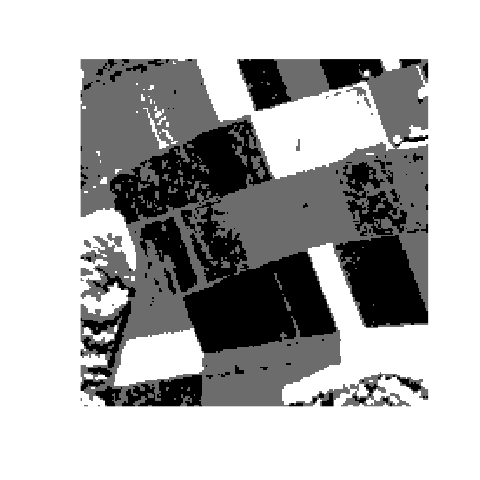
\includegraphics[scale=0.6]{3-01.png}
  \caption{$K=3$ and $\tau=0.1$.}
\end{figure}
\begin{figure}[!ht]
  \centering
    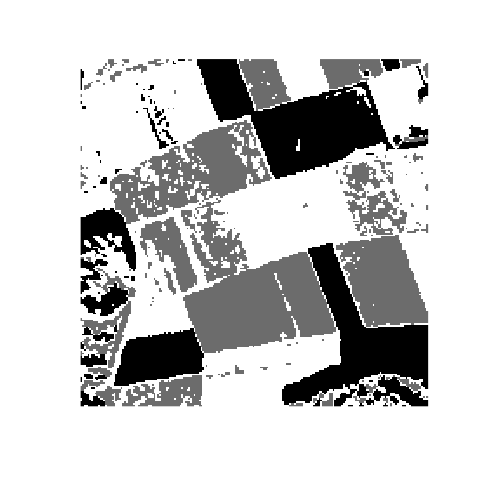
\includegraphics[scale=0.6]{3-001.png}
  \caption{$K=3$ and $\tau=0.01$.}
\end{figure}
\begin{figure}[!ht]
  \centering
    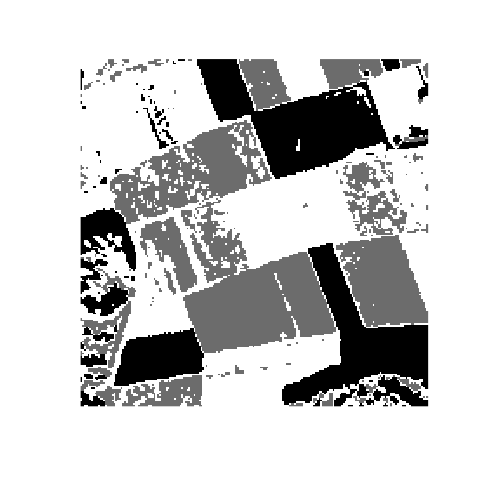
\includegraphics[scale=0.6]{3-0001.png}
  \caption{$K=3$ and $\tau=0.001$.}
\end{figure}
\begin{figure}[!ht]
  \centering
    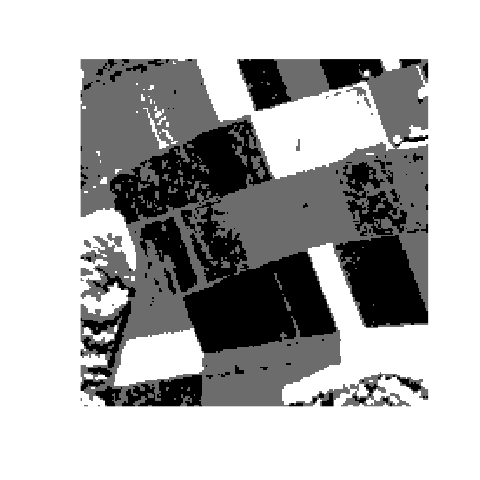
\includegraphics[scale=0.6]{3-00001.png}
  \caption{$K=3$ and $\tau=0.0001$.}
\end{figure}
\begin{figure}[!ht]
  \centering
    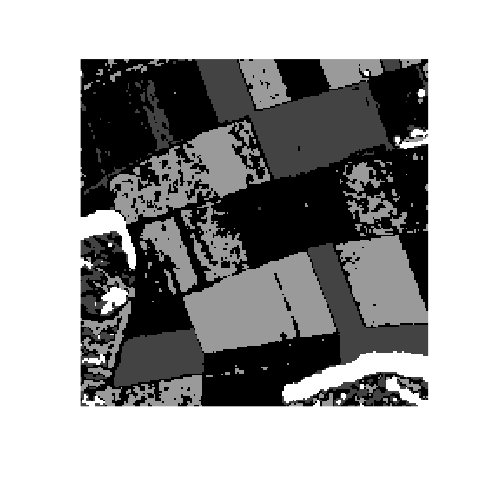
\includegraphics[scale=0.6]{4-01.png}
  \caption{$K=4$ and $\tau=0.1$.}
\end{figure}
\begin{figure}[!ht]
  \centering
    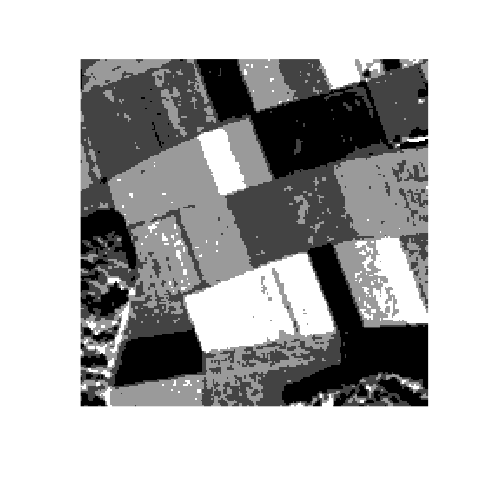
\includegraphics[scale=0.6]{4-001.png}
  \caption{$K=4$ and $\tau=0.01$.}
\end{figure}
\begin{figure}[!ht]
  \centering
    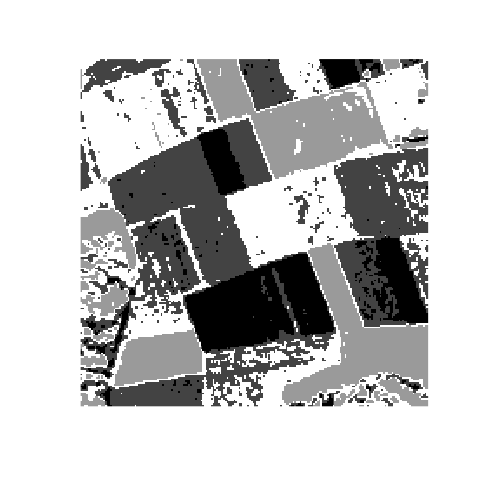
\includegraphics[scale=0.6]{4-0001.png}
  \caption{$K=4$ and $\tau=0.001$.}
\end{figure}
\begin{figure}[!ht]
  \centering
    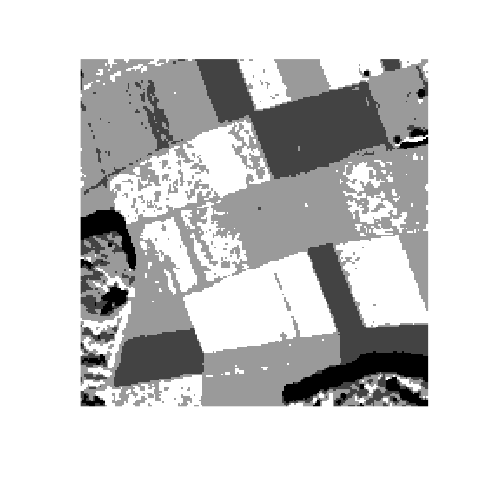
\includegraphics[scale=0.6]{4-00001.png}
  \caption{$K=4$ and $\tau=0.0001$.}
\end{figure}
\begin{figure}[!ht]
  \centering
    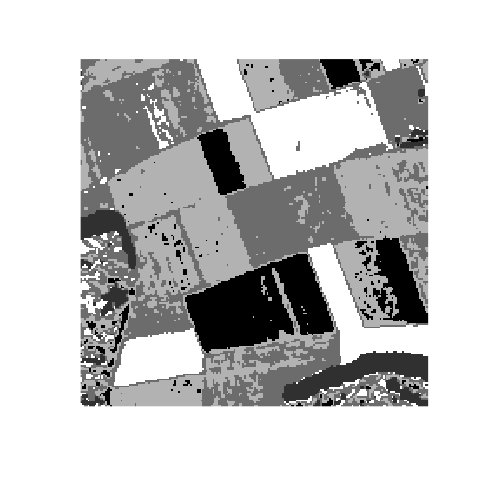
\includegraphics[scale=0.6]{5-01.png}
  \caption{$K=5$ and $\tau=0.1$.}
\end{figure}
\begin{figure}[!ht]
  \centering
    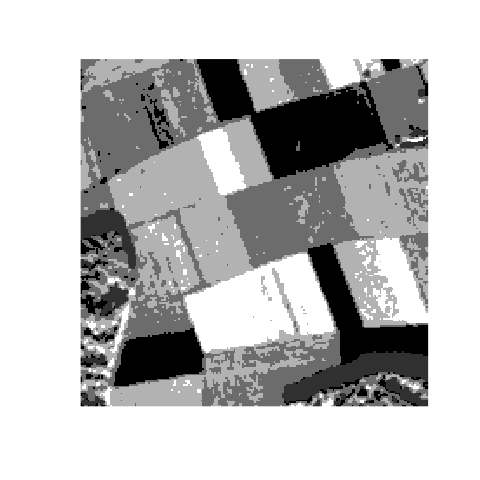
\includegraphics[scale=0.6]{5-001.png}
  \caption{$K=5$ and $\tau=0.01$.}
\end{figure}
\begin{figure}[!ht]
  \centering
    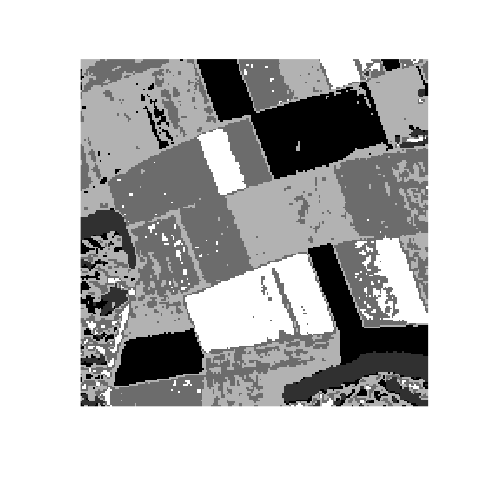
\includegraphics[scale=0.6]{5-0001.png}
  \caption{$K=5$ and $\tau=0.001$.}
\end{figure}
\begin{figure}[!ht]
  \centering
    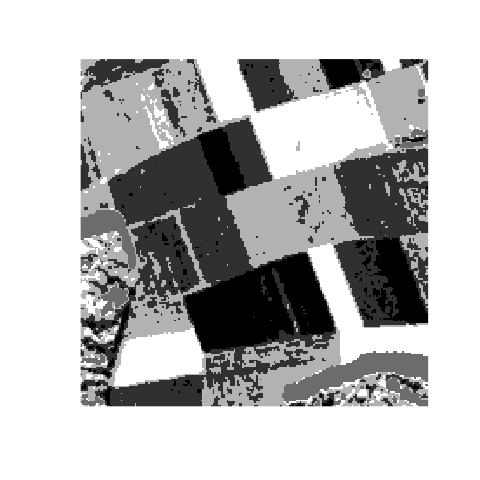
\includegraphics[scale=0.6]{5-00001.png}
  \caption{$K=5$ and $\tau=0.0001$.}
\end{figure}
\end{document} 